\section{Discussion}
\label{sec:discussion}

\subsection{Validating Structural Reasoning}

Five-phase validation provides evidence that the LLM performs structural reasoning rather than pattern matching. The 69.1 percentage point discrimination between 2024 (81.2\%) and 2020 (12.1\%) establishes selectivity: if the model relied on memorized associations or universal statistical patterns, detection rates would converge across periods rather than exhibiting 5.7$\times$ separation.

Three findings support this interpretation. First, the LLM maintained 98\% mechanical accuracy across both detection conditions---correctly computing persistence, magnitude, and flip counts regardless of whether windows qualified as regimes. Second, negative controls achieved 0\% false positives on transitional and low-magnitude synthetic data, confirming the model enforces structural criteria rather than over-detecting patterns. Third, confidence scores provide continuous quality discrimination beyond binary classification ($r > 0.4$ with regime metrics), suggesting the model tracks regime robustness, not just threshold crossing.

This selectivity contrasts with earlier 5-day trajectory testing~\cite{regan2025obfuscation}, which achieved 98--100\% detection across all market conditions by identifying universal daily hedging flows. The deliberate shift to 30-day windows with strict criteria transformed the task from universal pattern matching to selective regime identification---a critical distinction for validating genuine structural reasoning.

\subsection{Structural Reasoning versus Rule Execution}

A reasonable concern is whether 98\% mechanical accuracy indicates rule execution rather than reasoning. We address this directly. The 69.1pp discrimination between 2020 and 2024 is a property of the temporal data, reproducible by any classifier applying our thresholds. Our contribution is not that the LLM outperforms a rule-based baseline; it is that temporal obfuscation validates whether the LLM can faithfully apply structural criteria under domain-specific contamination risk. Agreement with rule-based thresholds is the validation signal, not a weakness. Beyond binary classification, the LLM produces outputs rules cannot: continuous confidence calibration ($r = +0.501$ with persistence, $r = -0.549$ with stability) and interpretable reasoning traces, with 88\% of sampled detections explicitly verifying criterion satisfaction step-by-step. The 2\% mechanical-accuracy gap reflects boundary-aware behavior on ambiguous windows (persistence within $\pm$0.02 of threshold) where reasoning traces acknowledged threshold proximity rather than forcing deterministic cutoffs.

\subsection{Market Structure Evolution}

The multi-year temporal analysis (Phase 5) reveals gradual regime evolution tracking 0DTE options adoption rather than sharp structural breaks. Detection progressed from 12.2\% (2020) through borderline years (3.7\% in 2021, 32.4\% in 2022) to sustained 100\% detection in 2024--2025, with GEX magnitude growing 360\% (\$5B $\rightarrow$ \$23B).

\begin{figure}[!htbp]
\centering
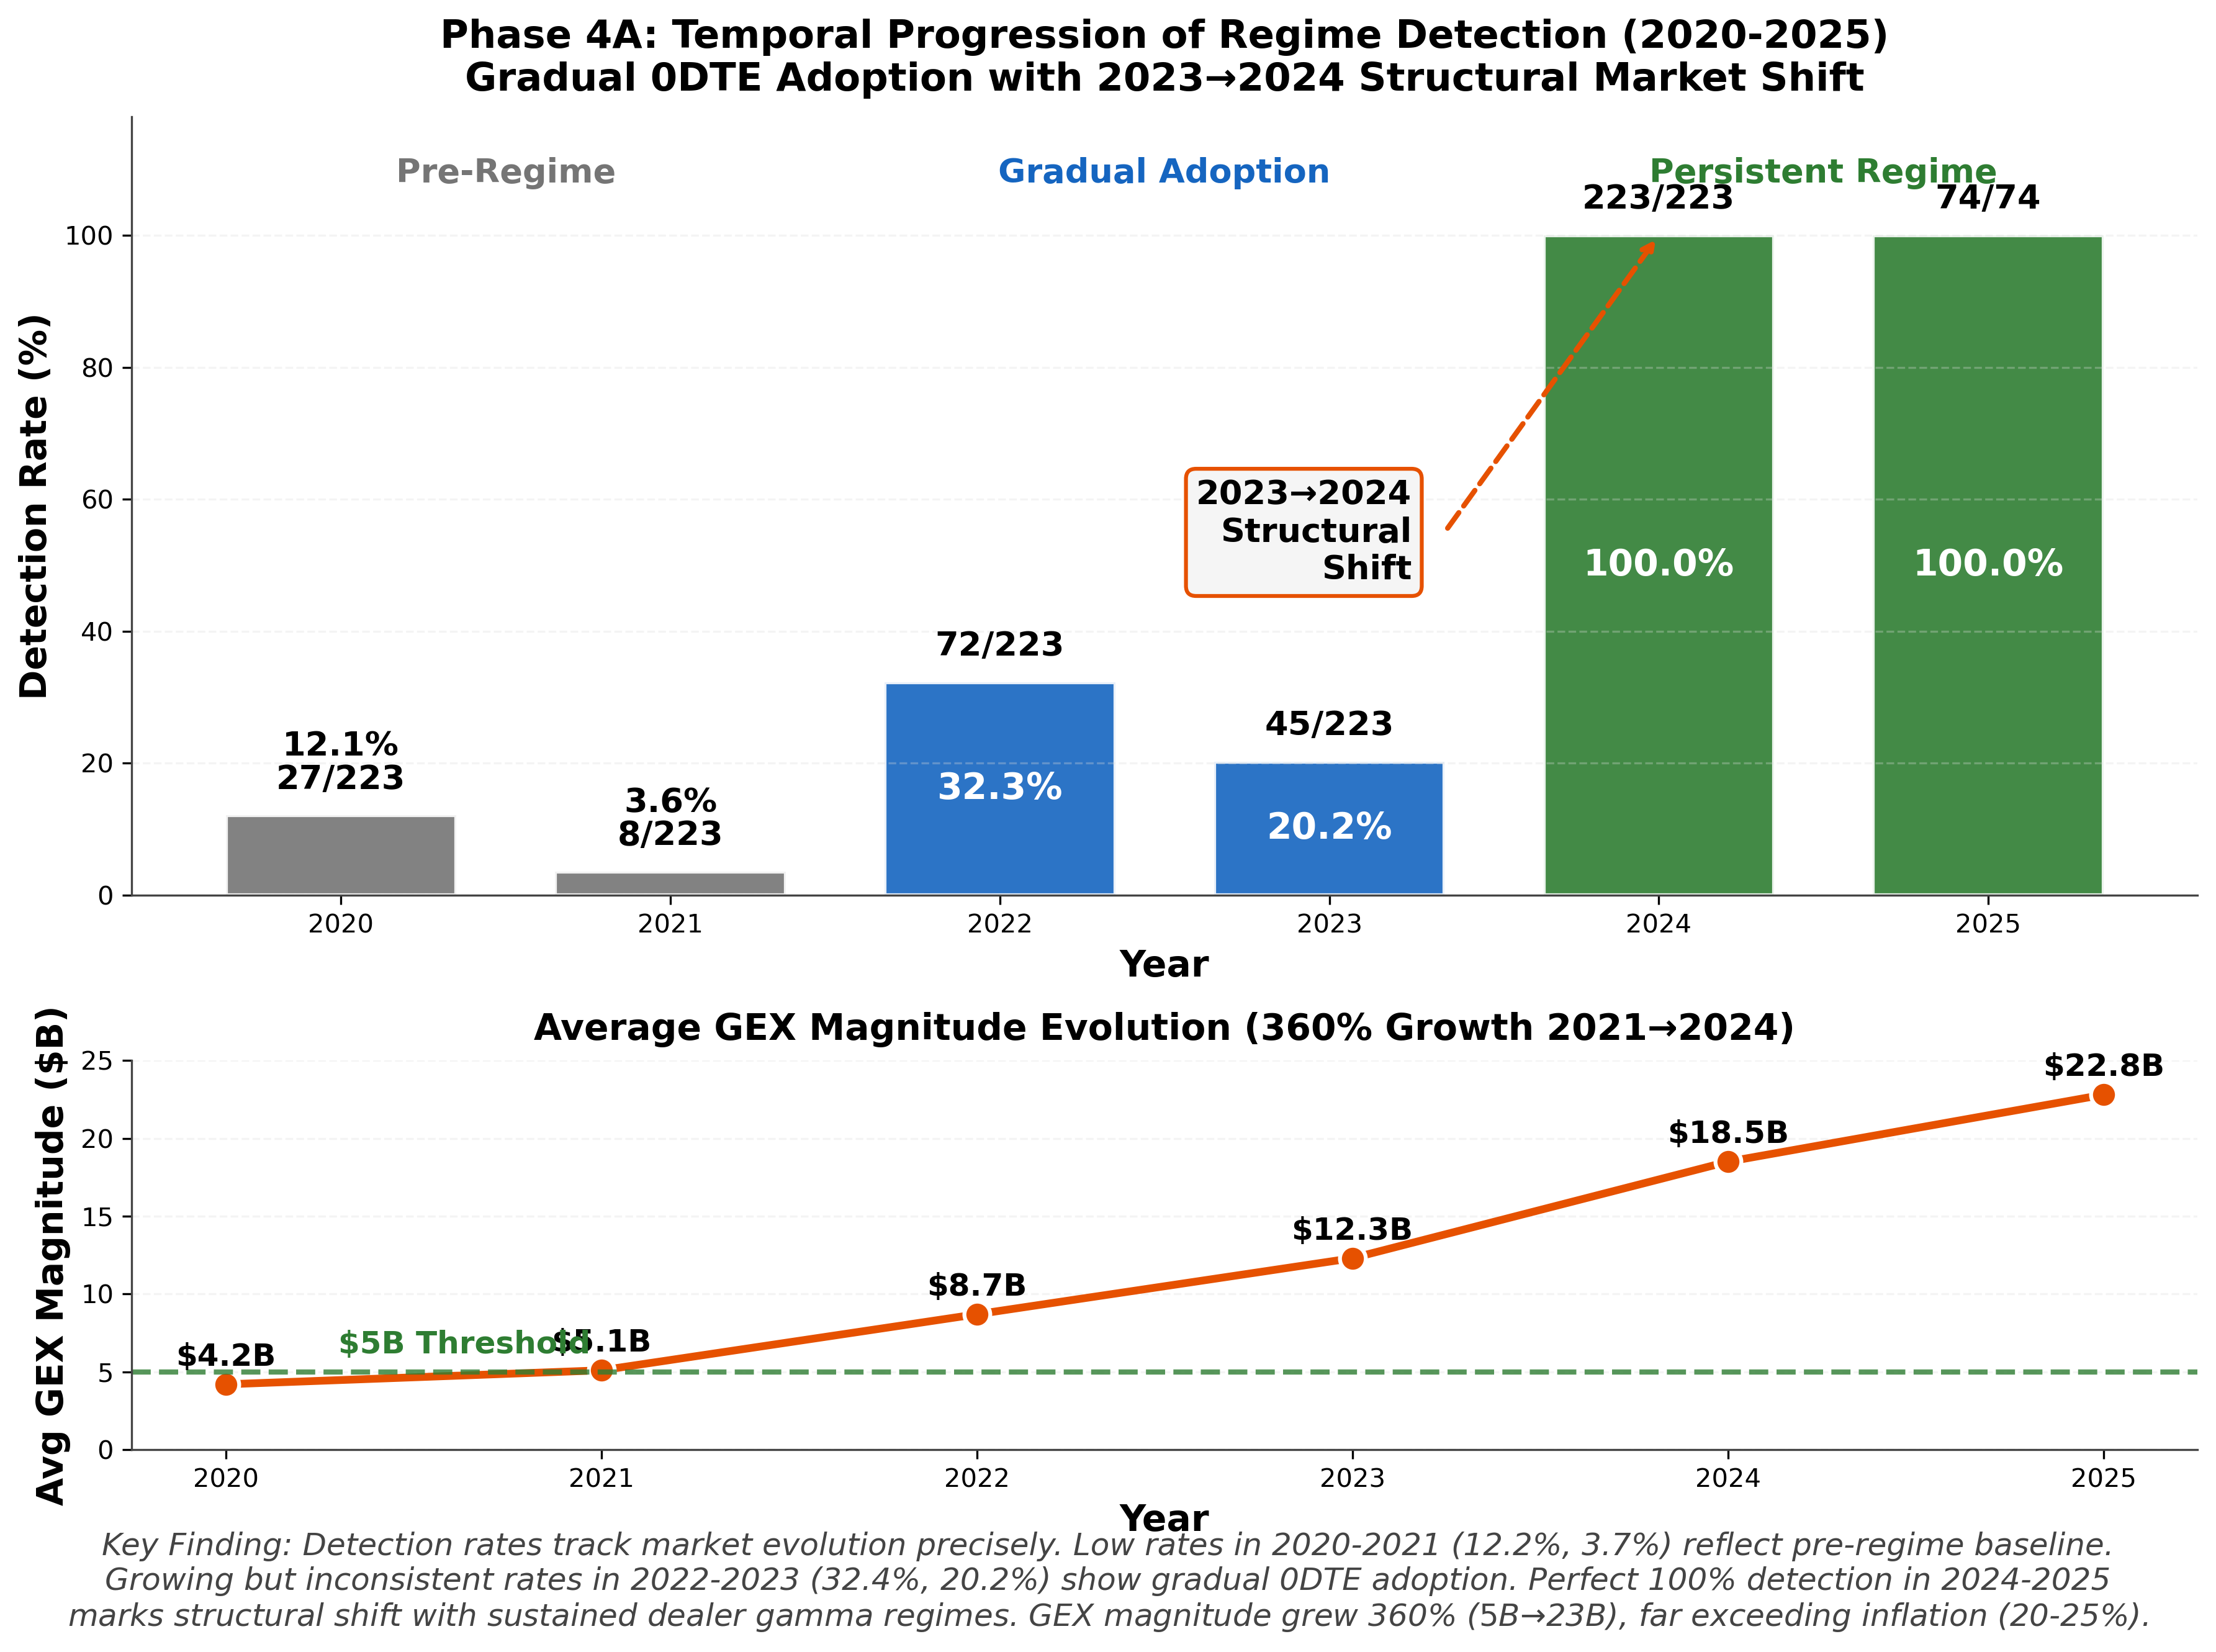
\includegraphics[width=\textwidth]{../figures/output/fig08_detection_progression.png}
\caption{Temporal progression of regime detection (2020--2025). Detection rates evolved from pre-regime baseline through growing adoption to structural shift at 100\% in 2024--2025. GEX magnitude grew 360\%, far exceeding inflation.}
\label{fig:progression}
\end{figure}

The non-monotonic pattern (32.4\% in 2022 dipping to 20.2\% in 2023 before reaching 100\% in 2024) is informative: 2023's elevated volatility (FOMC uncertainty, banking stress) repeatedly disrupted regime formation despite growing 0DTE hedging pressure, suggesting regime persistence requires both sustained dealer pressure \textit{and} a volatility environment permitting consolidation. This tipping-point dynamic strengthens the structural interpretation.

While the temporal coincidence with 0DTE proliferation is consistent with a causal relationship, we acknowledge that concurrent factors---interest rate changes (0.25\% $\rightarrow$ 5.5\%), volatility regime shifts, quantitative trading growth, and market maker concentration---may contribute. However, the non-monotonic detection pattern argues against gradual secular trends as primary drivers: detection remained flat through 2023 despite continuous interest rate increases and technology diffusion, then jumped discontinuously in 2024 coinciding with 0DTE market saturation ($\approx$48\% volume share).

\subsection{Temporal Obfuscation as Generalizable Methodology}

Our obfuscation testing framework generalizes beyond financial applications. The core principle---stripping temporal and contextual identifiers to force structural reasoning---addresses a universal challenge in deploying LLMs for domain-specific analysis: distinguishing genuine reasoning from training data contamination. The methodology requires three components: (1) identifiable features that can be systematically removed, (2) structural patterns that persist after obfuscation, and (3) negative controls validating discrimination.

Potential applications include medical time series analysis (removing patient identifiers and dates while preserving physiological patterns), climate data analysis (obfuscating location and temporal markers), and industrial anomaly detection (stripping equipment identifiers). In each case, temporal obfuscation could validate whether LLMs reason from structural properties or rely on memorized associations from training data.

\subsection{Limitations and Future Work}

Five limitations merit discussion, each pointing to concrete next steps.

\noindent\textbf{Single asset}: Testing focused on SPY; cross-asset generalization (individual equities) remains untested. Future work will extend the framework to high-volume equity options (e.g., AAPL, NVDA) and index alternatives (QQQ, IWM) to test whether regime detection reflects market-wide versus asset-specific dealer dynamics.

\noindent\textbf{End-of-day measurement}: Our GEX\_OI approach captures dealer inventory but not intraday gamma dynamics; integrating high-frequency order flow data would enable within-day regime transitions and sharpen the structural signal.

\noindent\textbf{Causal attribution}: The 0DTE hypothesis is supported by temporal coincidence and theoretical mechanism but remains circumstantial; observational data cannot exclude alternative explanations. Natural experiments around 0DTE rule changes or cross-market comparisons (SPX vs NDX expiration expansion) could provide quasi-experimental evidence.

\noindent\textbf{Framework-dependent reasoning}: Ablation testing (n=84) confirmed identical classification accuracy with and without narrative scaffolding. Future evaluation across multiple LLM architectures (Anthropic Claude, Google Gemini) would test whether obfuscated detection transfers across reasoning paradigms.

\noindent\textbf{Threshold sensitivity}: All 25 tested parameter combinations maintained $>$72pp discrimination, but thresholds represent empirically validated design choices rather than first-principles derivations. Deriving thresholds from equilibrium dealer-hedging models would strengthen theoretical grounding.
